\section{14.10.2014 - Raddrizzatore, Amplificatori e Termoresistenza}

In questa esperienza progetteremo un raddrizzatore di precisione (utilizzabile anche per segnali di bassa tensione). Dopodiché valuteremo la capacità di un amplificatore differenziale e dell'integrato $AD622$ di abbattere i guadagni in modo comune. Infine utilizzeremo una termoresistenza per misurare la temperatura.

\subsection*{Strumenti e materiali}

\begin{itemize} [noitemsep]
\item Oscilloscopio Agilent DSO-X 2002A (bandwidth \SI{70}{\mega\hertz}, sample rate \num{2} GSa/s);
\item Generatore di tensione continua Agilent E3631A (max $\pm \, \SI{25}{\volt}$ o $\pm \, \SI{6}{\volt}$);
\item Generatore di forme d'onta Agilent 33120A con range di frequenza da \SI{100}{\micro\hertz} a \SI{15}{\mega\hertz};
\item Multimetro Agilent 34410A a sei cifre e mezza;
\item Un amplificatore operazionale $\mu$A741;
\item Un integrato AD622;
\item Una termoresistenza PT100;
\item Resistenze e capacità di vari valori;
\item Due trimmer multigiro da \SI{10}{\kilo\ohm};
\item Breadboard e cablaggi vari.
\end{itemize}

\subsection{Raddrizzatore di precisione}

%\subsubsection*{Premessa sui raddrizzatori}

%I raddrizzatori sono dei circuiti il cui scopo è quello di effettuare il modulo di un segnale in ingresso preservandone la forma. In precedenti corsi di optoelettronica abbiamo incontrato alcuni semplici raddrizzatori i cui elementi circuitali chiave erano i diodi. Questi dispositivi sono in grado di portarsi in conduzione, e quindi di chiudere il ramo di circuito in cui si è posto il diodo, se la tensione al polo positivo è maggiore di quella al polo negativo; altrimenti il diodo apre il circuito. In realtà, ciò accade unicamente nel caso in cui il diodo sia ideale: per polarizzare un diodo è infatti necessario creare una differenza di tensione ai suoi capi, detta tensione di soglia $V_d$, che ha un valore di $\approx 0.6$ \si{\volt}; altrimenti il diodo risulterà come non polarizzato e dunque non in conduzione. Questo fatto, nella creazione di raddrizzatori può creare alcuni svantaggi, soprattutto se necessaria un'alta precisione (lavorando con piccoli valori di tensione): il segnale in uscita sarà con la stessa forma d'onda del segnale in entrata, ma con un offset di $-0.6$\si{\volt} dato dalla $V_d$; inoltre, se i segnali in entrata hanno valori più piccoli della tensione di soglia, il diodo non entrerà mai in conduzione. Di seguito presentiamo alcuni circuiti che risolvono in parte queste problematiche.

\subsubsection{Raddrizzatore}

\begin{wrapfigure}[16]{r}{0.5\textwidth}
  \begin{center}
    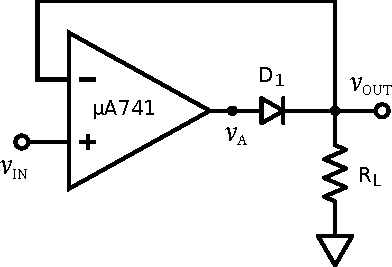
\includegraphics[width=0.350\textwidth]{../E05/latex/c_rectifier_A.pdf}
  \end{center}
  \caption{Circuito del raddrizzatore con un diodo. La resistenza di carico è $R_L=10$ \si{\kilo\ohm}.}
  \label{cir5:raddrizz_1}
\end{wrapfigure}

Analizziamo il circuito in Figura \ref{cir5:raddrizz_1}. Vogliamo dimostrare che, qualunque sia il segnale in entrata, il contributo alla tensione di uscita dato dalla tensione di soglia del diodo è trascurabile.

Innanzitutto notiamo che, dato l'alto guadagno dell'operazionale, la tensione in entrata per polarizzare il diodo è un valore molto basso (con un guadagno di $2\times 10^5$ la tensione necessaria è data da $0.6 \si{\volt}/2\times 10^5 \approx 3 \si{\micro\volt}$); dunque non dobbiamo preoccuparci che il segnale in entrata debba avere un valore minimo per far funzionare il circuito.

Vale per l'operazionale l'equazione (\ref{eq3:regola_opamp})\footnote{In realtà bisognerebbe considerare anche la dipendenza dalla frequenza. Abbiamo però notato che, ben prima che si possa apprezzare l'abbattimento dell'amplificazione, incorreremo in un altro problema dato dalla velocità di polarizzazione dei transistor all'interno dell'operazionale che ci porterà a scartare questo circuito come raddrizzatore di precisione ad alte frequenze.}
\begin{equation}
V_{A}=A (V^+-V^-)
\label{eq5:regola_opamp_NOFREQDEP}
\end{equation}
dove $V_{A}$ è la tensione all'uscita dell'amplificatore operazionale.
Valutiamo ora il circuito in due casi: $V_{in}<0$ e $V_{in}>0$\footnote{Grazie alle considerazioni sopra possiamo trascurare la tensione in ingresso necessaria per polarizzare il diodo}.

\paragraph*{Caso $V_{in}<0$}

Nel primo caso, l'OPAMP amplifica il segnale negativo in entrata sull'uscita rispettando la (\ref{eq5:regola_opamp_NOFREQDEP}) con $V_-=0$: infatti, essendo il diodo interdetto (il polo positivo è più negativo di quello negativo), non passa alcuna corrente per $R_L$ rendendo $V^-=V_{out}=0$. Inoltre, dato che l'OPAMP è in saturazione ($V^+-V^-$ diventa molto grande), $V_A \approx V_{CC}$.

\paragraph*{Caso $V_{in}>0$}

Nel secondo caso invece il diodo è in conduzione. Consideriamo dunque, come si nota dalla Figura \ref{cir5:raddrizz_1}
$$V^+=V_{in} \qquad V^-=V_{out}$$
Dato che un diodo in conduzione ha una caduta in buona approssimazione costante $V_d$, vale anche che
$$V_{A}=V_{out}+V_d$$
Sostituendo questi risultati in (\ref{eq5:regola_opamp_NOFREQDEP}) otteniamo le equazioni cercate
\begin{equation}
V_{out}=\frac{1}{1+A} (A V_{in} - V_d) \approx V_{in} \qquad V_{A} \approx V_{in}+V_d
\label{eq5:leggi_1.1}
\end{equation}

In Figura \ref{gr5:primo_raddrizzatore} presentiamo i grafici delle tensioni in funzione del tempo alla frequenza di $50$ \si{\hertz}.

\begin{figure}[H]
 \centering
   {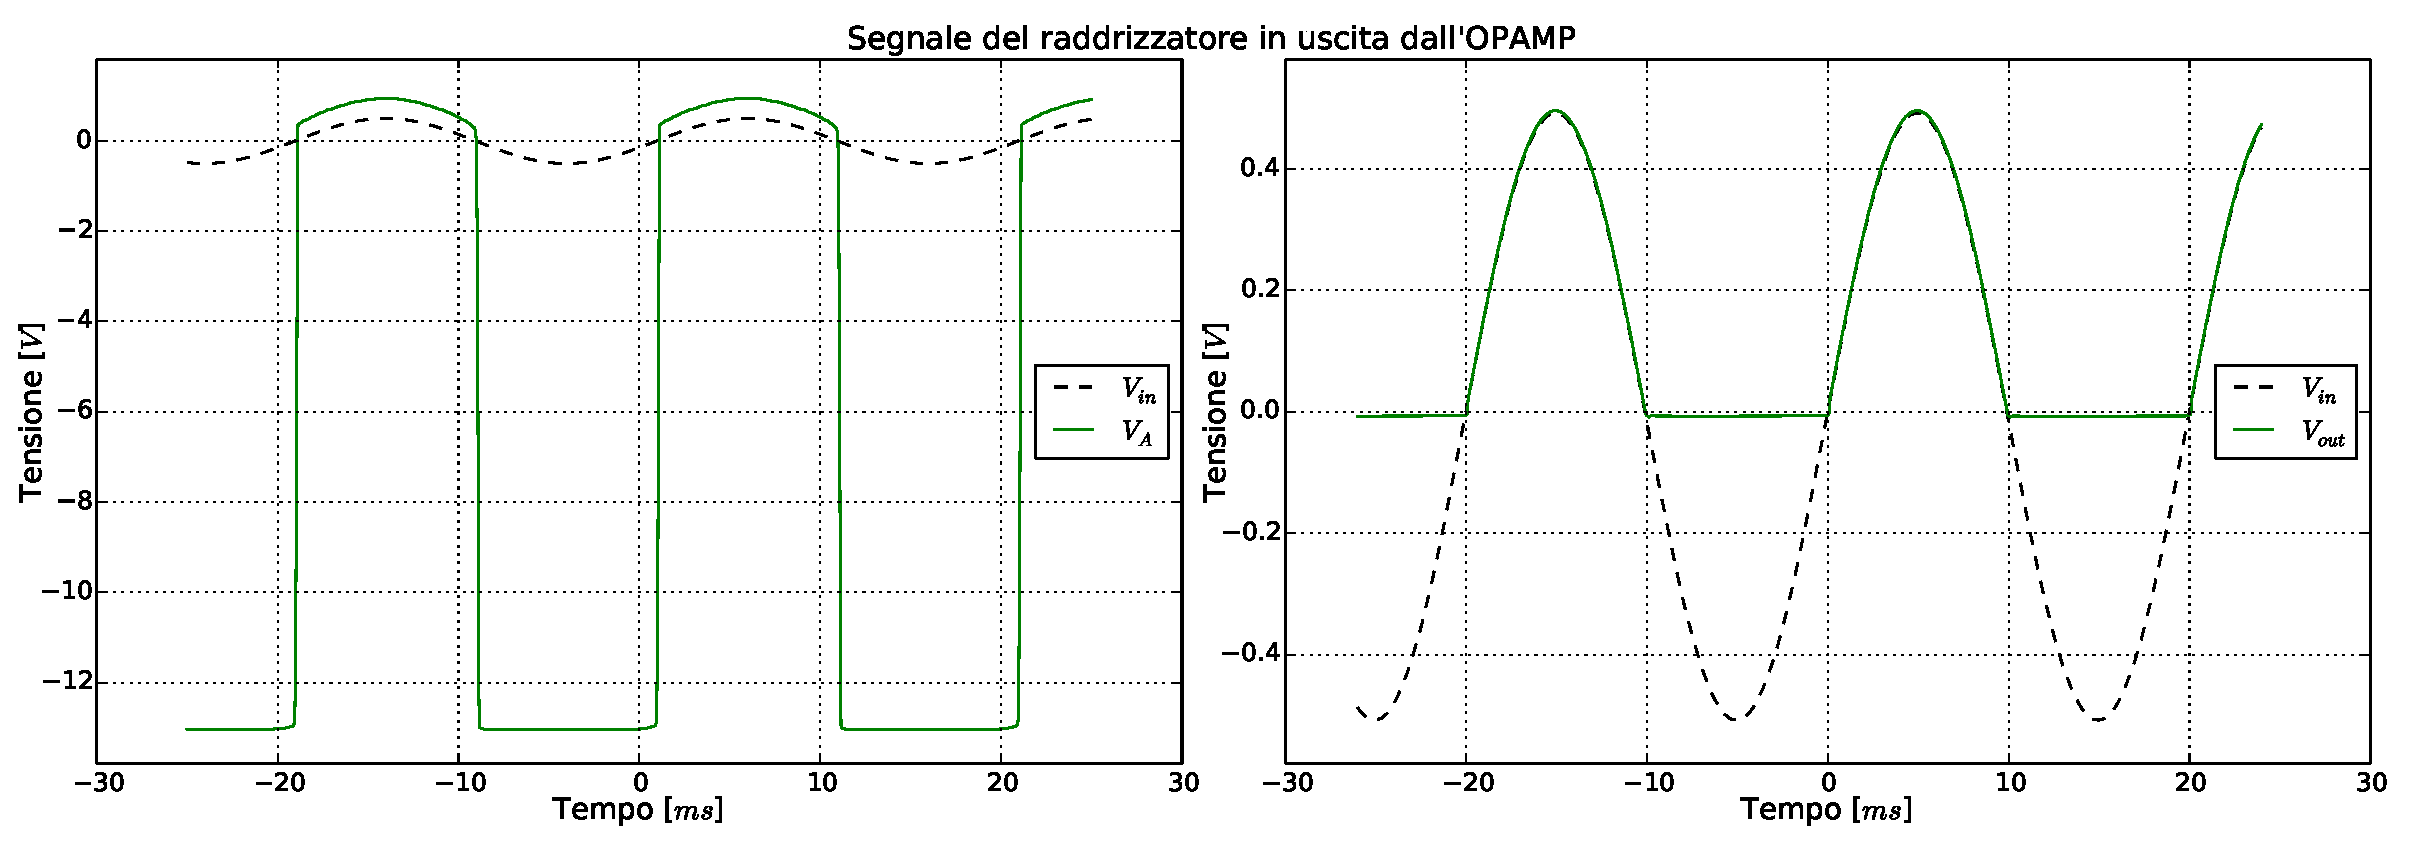
\includegraphics[width=16.5cm]{../E05/latex/unite_tempo.pdf}}
 \caption{Grafici delle tensioni in funzione del tempo. Il primo grafico è quello relativo alla tensione all'uscita del circuito $V_{out}$, il secondo alla tensione in uscita dall'OPAMP $V_A$, dove è facile vedere che l'operazionale entra in saturazione negativa.}
 \label{gr5:primo_raddrizzatore}
\end{figure}

In Figura \ref{gr5:primo_raddrizzatore_vin} presentiamo invece i grafici delle tensioni come funzioni di $V_{in}$

\begin{figure}[H]
 \centering
   {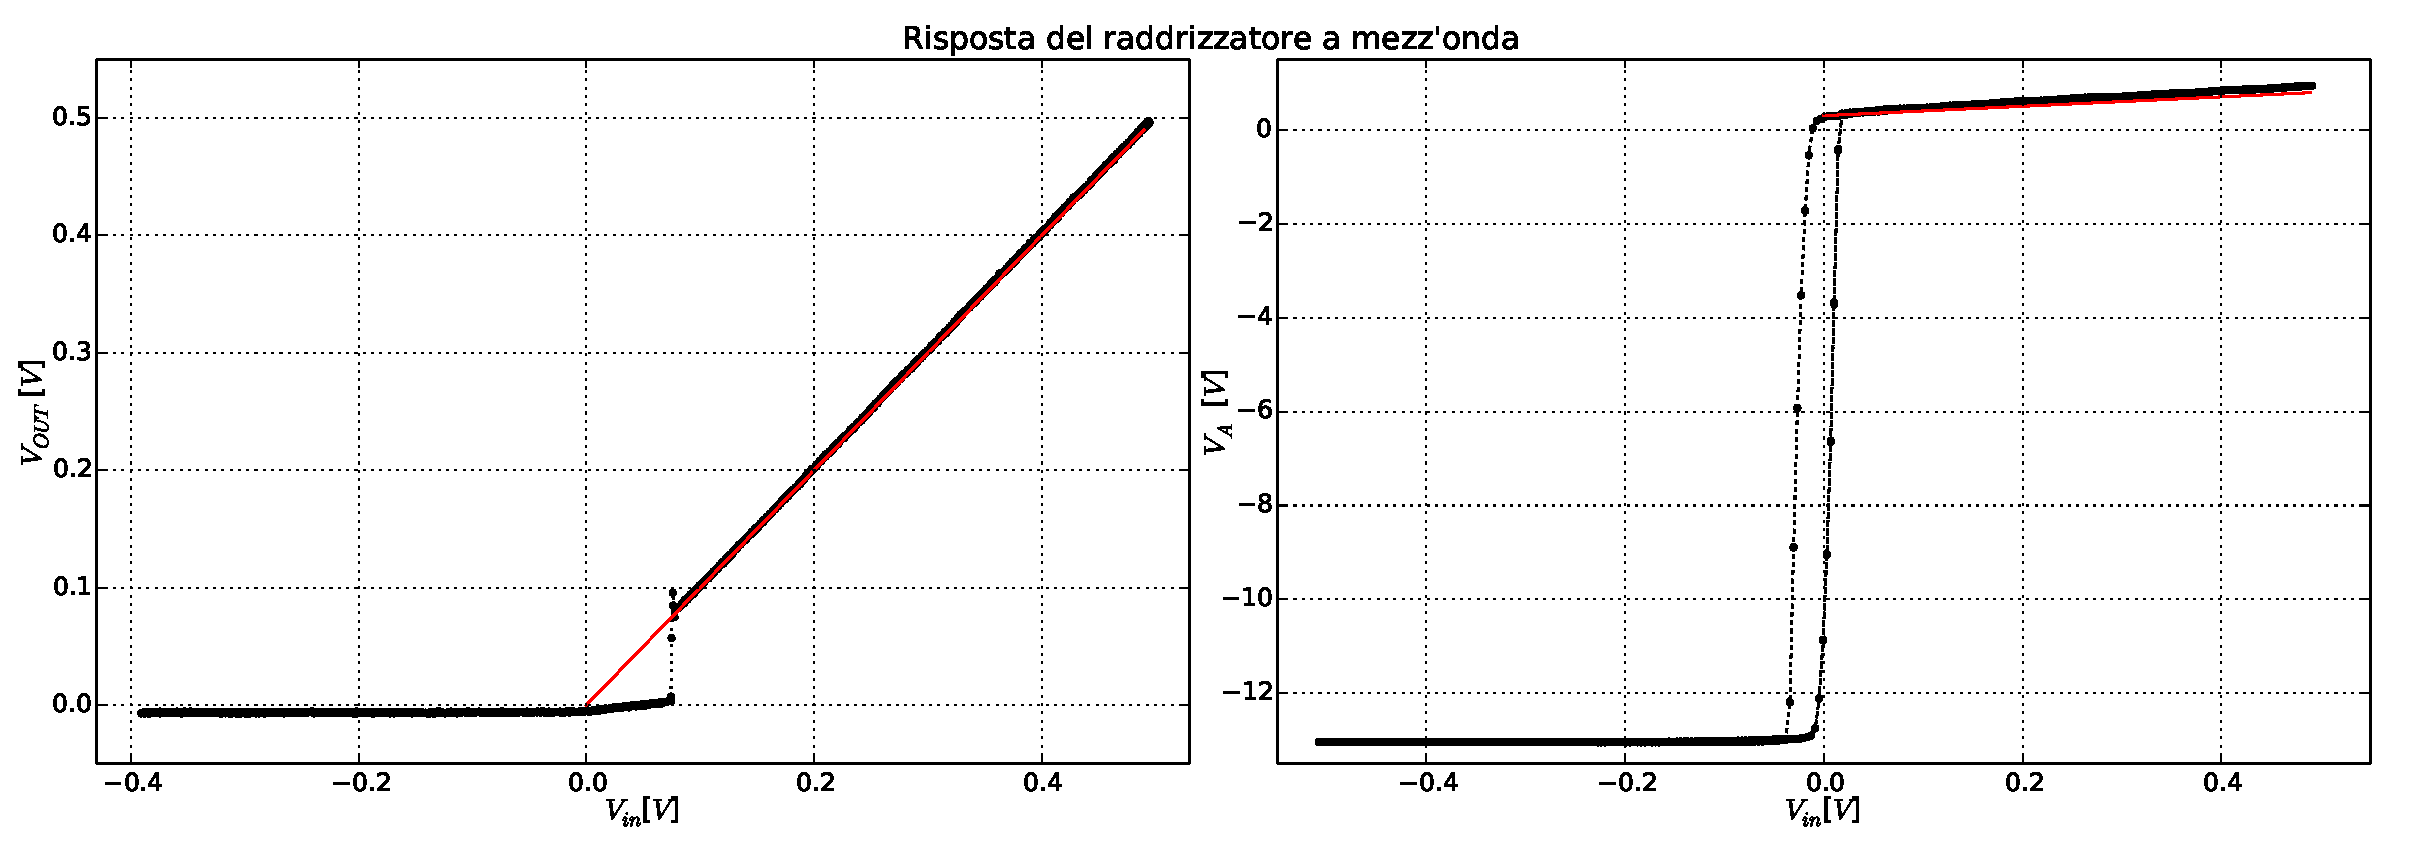
\includegraphics[width=16.5cm]{../E05/latex/u_risposta.pdf}}
 \caption{Grafici rispettivamente (da sinistra a destra) della tensione in uscita dal circuito in funzione della tensione in entrata, e della tensione in uscita dall'OPAMP in funzione della tensione in ingresso.}
 \label{gr5:primo_raddrizzatore_vin}
\end{figure}

\begin{figure}[H]
 \centering
   {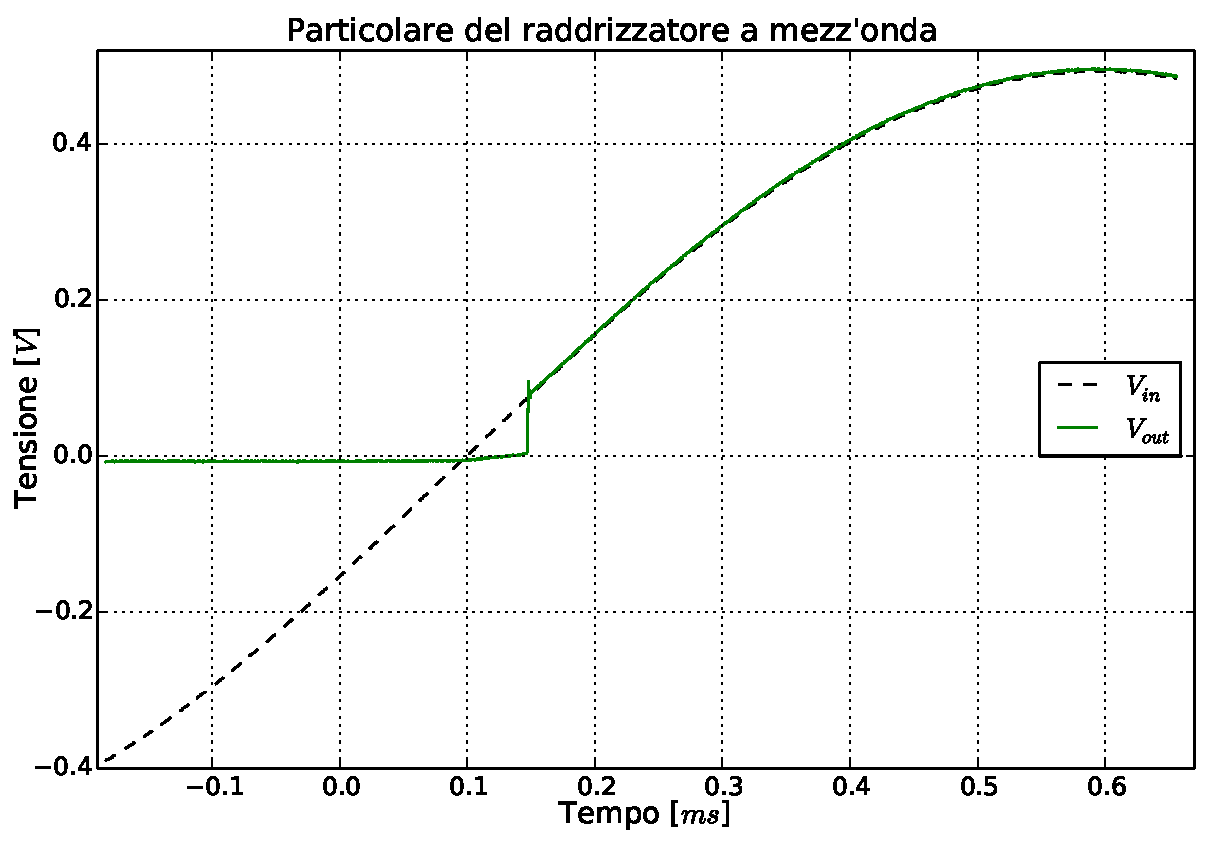
\includegraphics[width=11.5cm]{../E05/latex/zoom.pdf}}
 \caption{Grafico della tensione in entrata (tratteggiata) e della tensione in uscita dal circuito (in verde) in funzione del tempo. Si nota il fenomeno esposto nel paragrafo.}
 \label{gr5:problema}
\end{figure}

Dal plot del segnale in entrata ed in uscita in funzione del tempo alla frequenza di 2 \si{\kilo\hertz} (grafico in Figura \ref{gr5:problema}), possiamo notare un troncamento della forma d'onda del segnale in uscita. Abbiamo ipotizzato che tale fenomeno fosse dovuto alla limitata velocità che i transistor all'interno dell'operazionale hanno di passare dalla saturazione all'interdizione; tale fenomeno è anche amplificato dal fatto che, quando il diodo è interdetto, $V_{A} \approx -V_{CC}$: il segnale deve quindi passare da una tensione di saturazione negativa alla tensione necessaria per raddrizzare il segnale in uscita in un tempo troppo breve, e ad alte frequenze ciò risulta in un troncamento. Per risolvere tale problema utilizziamo il circuito esposto al sottoparagrafo successivo.

\subsubsection{Raddrizzatore ottimizzato}

\begin{wrapfigure}[16]{l}{0.5\textwidth}
  \begin{center}
    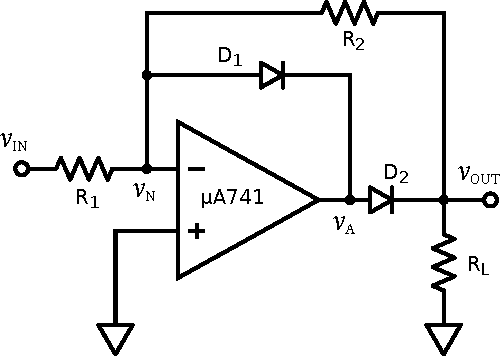
\includegraphics[width=0.350\textwidth]{../E05/latex/c_rectifier_B.pdf}
  \end{center}
  \caption{Circuito del raddrizzatore a semionda ottimizzato. La resistenza di carico è $R_L=10$ \si{\kilo\ohm}, mentre $R_1=R_2=10$ \si{\kilo\ohm}.}
  \label{cir5:raddrizz_2}
\end{wrapfigure}

Per risolvere il problema visto in precedenza, utilizziamo un secondo diodo posto come nel in Figura \ref{cir5:raddrizz_2} e un circuito di retroazione controllata in guadagno. Anche in questo caso dobbiamo valutare la risposta del circuito in casi diversi: $V_{in}=0$, $V_{in}>0$ e $V_{in}<0$.

\paragraph*{Caso $V_{in}=0$}

Nel primo caso abbiamo entrambi i diodi interdetti. Infatti, se la tensione in ingresso è nulla non vi è la tensione necessaria a polarizzare i diodi, che rimangono non polarizzati. Dunque $V_{out}=V_{A}=0$.

\paragraph*{Caso $V_{in}>0$}

Tenendo conto della (\ref{eq5:regola_opamp_NOFREQDEP}), considerando che $V_{in}$ viene portata sull'ingresso invertente, la tensione su $V_{A}$ sarà negativa e quindi più bassa di $V_{out}$: dunque $D_2$ sarà interdetto. Allo stesso tempo il polo positivo di $D_1$ è più positivo (a comune virtuale) di quello negativo ($V_{A}$), dunque tale diodo risulta in conduzione. Inoltre, $V_{out}$ risulta nulla in quanto sul ramo di circuito identificato da $R_2$ e $R_L$ non passa corrente (sono collegate rispettivamente a comune virtuale e comune). $V_{A}$ sarà invece fissata dalla tensione di soglia del diodo, cioè $V_{A}=-V_d$.

\paragraph*{Caso $V_{in}<0$}

Con considerazioni analoghe al caso precedente, possiamo concludere che $D_1$ risulta interdetto, mentre $D_2$ in conduzione. Quindi il circuito è un amplificatore invertente di segnale con guadagno $-R_2/R_1$.

Valutiamo il contributo del diodo nella tensione di uscita del circuito $V_{out}$ e dell'operazionale $V_{A}$. Consideriamo le correnti nel nodo $V_N$
$$\frac{V_{in}-V_N}{R_1} + \frac{V_{out}-V_N}{R_2} = 0$$
Osservando che $V_N$ è a ground virtuale, che $V_{out}=V_{A}-V_d$, e considerando l'operazionale come ideale e che vale che $V_{out}=V_{A}-V_d$, dalla (\ref{eq5:regola_opamp_NOFREQDEP}) otteniamo
\begin{equation}
V_{out}=-\frac{R_2}{R_1}V_{in} \qquad V_A = \frac{R_2}{R_1} V_{in} + V_d
\label{eq5:v_out_ottimizzato}
\end{equation}

In Figura \ref{gr5:secondo_raddrizzatore} presentiamo il grafico della tensione.

\begin{figure}[H]
 \centering
   {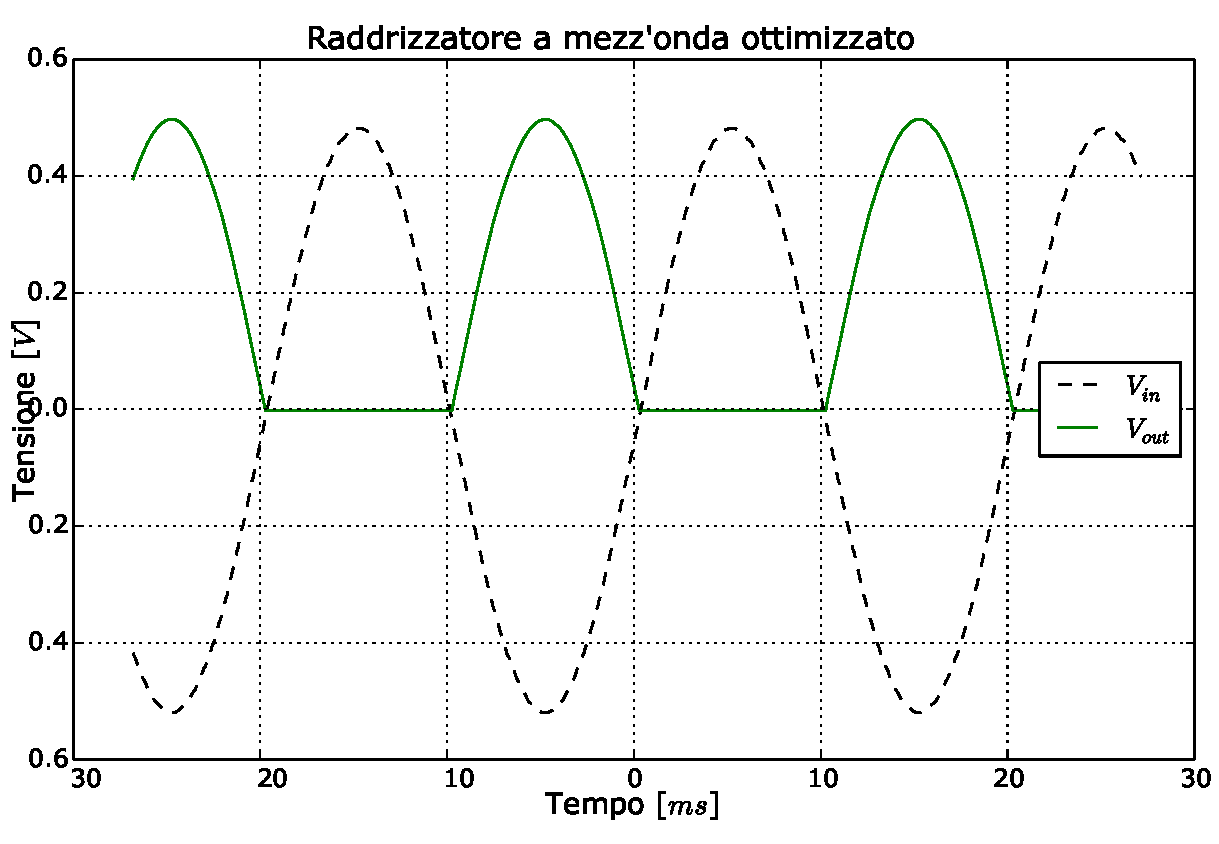
\includegraphics[width=11.5cm]{../E05/latex/radd_ott.pdf}}
 \caption{Grafico delle tensioni in funzione del tempo. Notiamo che il guadagno negativo quando $V_{in}<0$, plausibile con (\ref{eq5:v_out_ottimizzato}).}
 \label{gr5:secondo_raddrizzatore}
\end{figure}

\subsection{Amplificatore differenziale}

\begin{wrapfigure}[14]{l}{0.5\textwidth}
  \begin{center}
    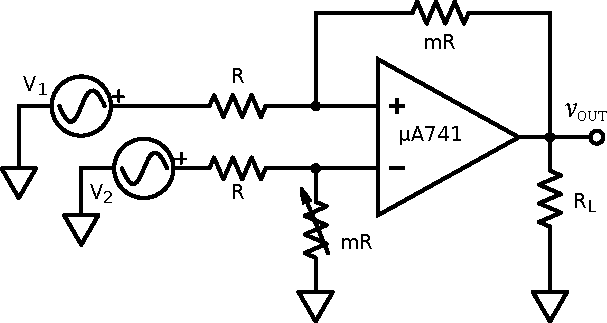
\includegraphics[width=0.33\textwidth]{../E05/latex/c_teo_diff_amp.pdf}
  \end{center}
  \caption{Schema circuitale di un amplificatore differenziale. Per $m$ si intende un fattore moltiplicativo rispetto alla $R$.}
  \label{cir5:diff_amp_teo}
\end{wrapfigure}

In questa parte dell'esperienza cercheremo di capire e analizzare un amplificatore differenziale, il cui schema circuitale è in Figura \ref{cir5:diff_amp}. Oltre al fatto che scegliendo i valori di resistenza possiamo decidere il guadagno, la proprietà più importante è sicuramente l'abbattimento del rumore di modo comune. Per capirne il motivo analizziamo il circuito teorico riportato in Figura \ref{cir5:diff_amp_teo}.

Sfruttiamo il principio di sovrapposizione per valutare la tensione in uscita in funzione delle due di ingresso, ricordandoci che tale principio può essere applicato per sistemi lineari: ciò è molto utile in quanto ci permette di separare l'analisi circuitale e ricondurci a casi più semplici.

Chiamiamo $V^-$ la tensione all'ingresso invertente e $V^+$ quella all'ingresso non invertente. Analizziamo prima il caso in cui $V_1=0$. La tensione nel punto $V_+$ sarà data dal partitore con $R$ ed $mR$ (verso l'op-amp non scorre corrente). Assumendo l'op-amp ideale, abbiamo $V^+=V^-$. Possiamo dunque scrivere:

\begin{equation}
\begin{cases} V_+=V_-  \\ V_+=V_2\frac{mR}{R+mR} \\ V_-= V_{out2}\frac{R}{R+mR}\end{cases}  \Rightarrow V_{out2}=mV_2
\label{eq 5: vout2}
\end{equation}

Analogamente, poniamo $V_2=0$. Otteniamo le seguenti equazioni del circuito:

\begin{equation}
\begin{cases} V_+=V_-=0  \\ \frac{V_1}{R}+\frac{V_{out2}}{mR}=0 \end{cases}  \Rightarrow V_{out1}=-mV_1
\label{eq 5: vout1}
\end{equation}

Sommando ora (\ref{eq 5: vout2}) e (\ref{eq 5: vout2}) otteniamo $V_{out}=m(V_2-V_1)$.

Possiamo ora passare ad analizzare il circuito da cui siamo partiti, ovvero quello affetto da noise (da noi simulato con un'onda sinusoidale) riportato in Figura \ref{cir5:diff_amp}. Valgono dunque le seguenti equazioni

%\begin{center}
$$
\begin{cases} V_1=V_{in}+V_{noise} \\ V_2=V_{noise} \end{cases}  \Rightarrow V_{out}=m(V_{noise}-(V_{in}+V_{noise}))=-V_{in}
$$
%\end{center}

L'amplificatore differenziale ci permette dunque di eliminare in modo efficace il rumore di modo comune. 

Inoltre, abbiamo posto come resistenza collegata tra comune e $V_+$ un trimmer per impostare la tensione di modo comune al più basso valore possibile. Infatti, le resistenze non sono in realtà esattamente uguali e prima di utilizzare il circuito è necessario bilanciarlo in modo da ottenere un segnale il più piccolo possibile quando i segnali in ingresso sono uguali.

\begin{wrapfigure}[17]{r}{0.5\textwidth}
  \begin{center}
    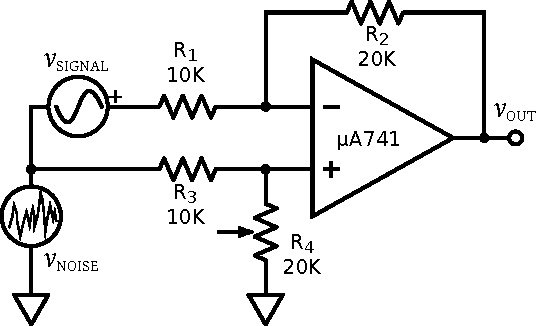
\includegraphics[width=0.33\textwidth]{../E05/latex/c_diff_amp.pdf}
  \end{center}
  \caption{Grafico dell'amplificatore differenziale utilizzato durante l'esperienza. $R_4$ è un trimmer multigiro di resistenza variabile.}
  \label{cir5:diff_amp}
\end{wrapfigure}

In laboratorio abbiamo utilizzato come sorgente di noise il generatore di forme d'onda e come $V_{in}$ il generatore di tensione costante. Abbiamo utilizzato delle R da \SI{10}{\kilo\ohm} e $mR=2R$. La resistenza variabile è stata costruita mettendo in serie una da \SI{10}{\kilo\ohm} con un trimmer, anch'esso da \SI{10}{\kilo\ohm}. Per controllare il bilanciamento abbiamo connesso entrambi gli ingressi al generatore di forme d'onda ed è stato utilizzato un segnale sinusoidale di $20Vpp$. Il segnale in uscita è stato dunque riportato sull'oscilloscopio. Abbiamo notato che, cambiando il valore della resistenza con il trimmer, il segnale in uscita variava. Il miglior bilanciamento che siamo riusciti a raggiungere ha portato la tensione picco-picco del rumore a \SI{0.5}{\milli\volt}. Abbiamo dunque posto come segnale in entrata un valore costante di tensione con il generatore di tensione costante, e alimentato il circuito con $-2Vpp$. Il rumore è sempre stato simulato con una sinusoidale di $20Vpp$. Questo risultato è riportato in Figura \ref{gr5:amp_diff}.

Come vediamo, il rumore è stato completamente eliminato dall'amplificatore differenziale. Abbiamo successivamente provato a sbilanciare il circuito, per vedere l'effetto del rumore sul segnale in uscita. E' stata dunque variata la resistenza con trimmer e abbiamo utilizzato un rumore con dei picchi molto accentuati, così da vedere bene gli effetti sul segnale in uscita (l'output è in Figura \ref{gr5:sbil_amp_diff}). 

\begin{figure}[H]
 \centering
   {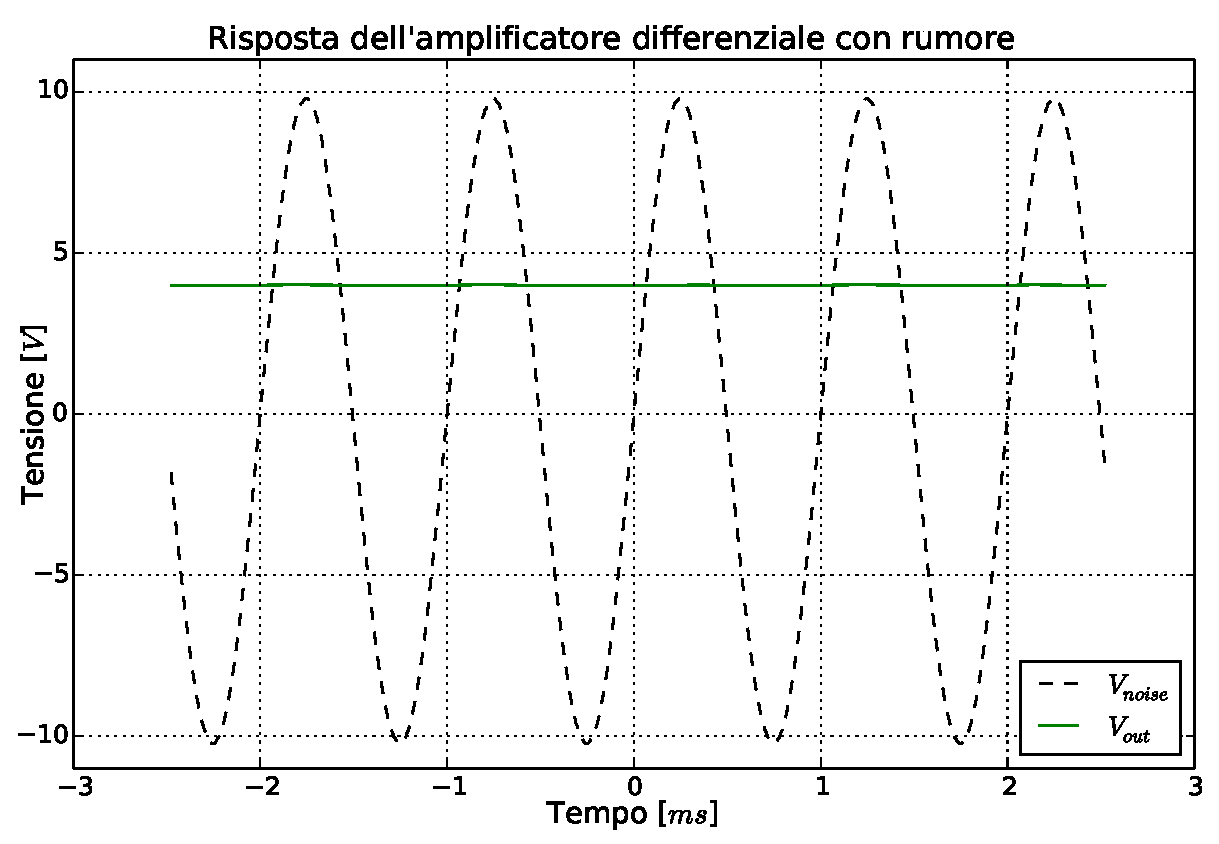
\includegraphics[width=0.7\textwidth]{../E05/latex/amp_diff.pdf}}
 \caption{Come vediamo dal grafico, il rumore che abbiamo simulato ha un'ampiezza di 20 Volt picco-picco (sinusoide in nero). Nonostante ciò, l'uscita (in verde) non è affatto influenzata e risulta amplificata di 2 volte, come stimato precedentemente dai calcoli teorici. }
 \label{gr5:amp_diff}
\end{figure}

\begin{figure}[H]
 \centering
   {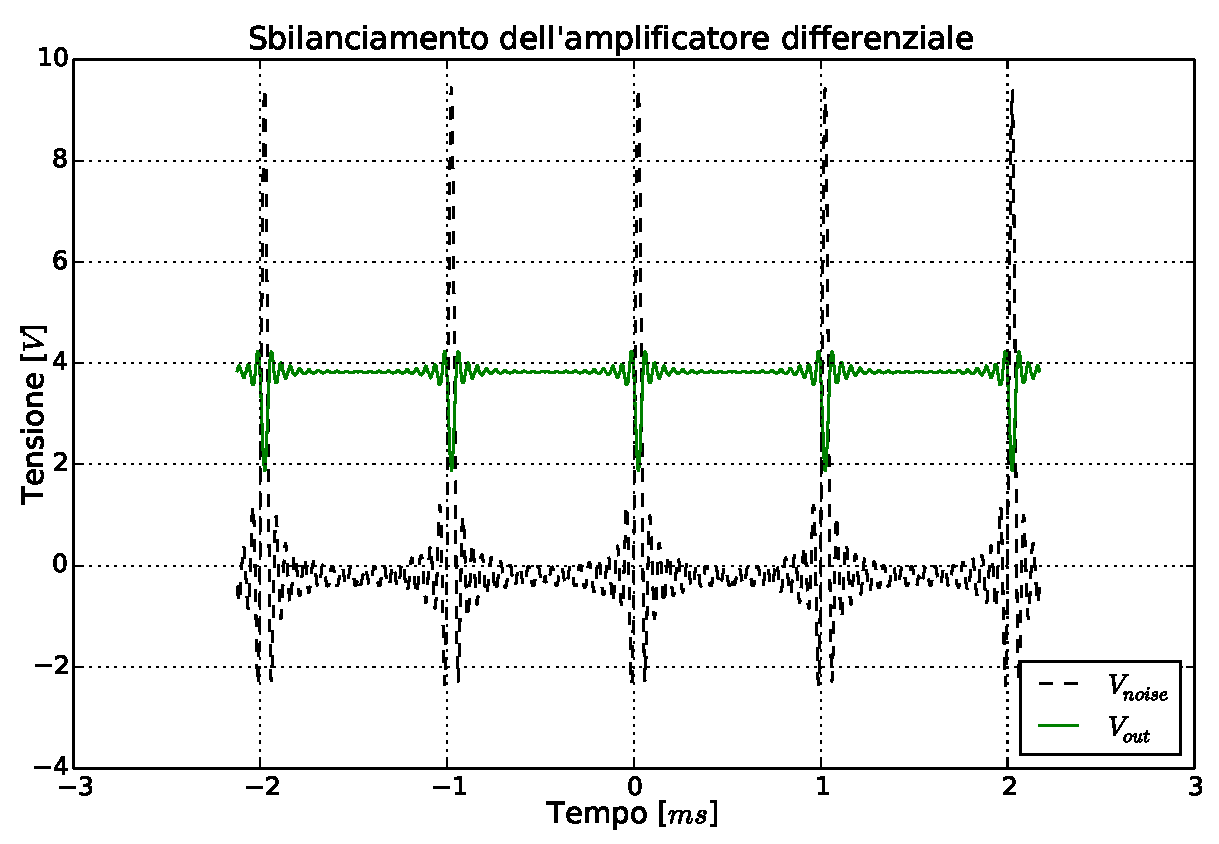
\includegraphics[width=0.7\textwidth]{../E05/latex/sbil_amp_diff.pdf}}
 \caption{Dopo lo sbilanciamento del circuito non è più garantita la soppressione del rumore in modo comune. Come vediamo, il segnale in uscita risulta distorto. E' dunque necessario calibrare bene il circuito prima di effettuare esperimenti nei quali si vuole eliminare un rumore comune ad entrambi i segnali in ingresso.}
 \label{gr5:sbil_amp_diff}
\end{figure}

Inoltre, il guadagno può essere cambiato solo se si cambiano 2 resistenze nel circuito. Una soluzione efficace che inoltre rimedia alla bassa impedenza in ingresso è quella di utilizzare un Amplificatore per Strumentazione, il cui funzionamento è esposto al paragrafo successivo.

\subsection{Amplificatore per Strumentazione}

\subsubsection*{Circuito didattico con opamp}



Il circuito visto al paragrafo precedente presenta dei problemi, nonostante abbatta in maniera abbastanza efficiente i segnali di modo comune. Per prima cosa l'impedenza in ingresso vista da un eventuale generatore di segnale è bassa, e ciò rende necessaria una potenza maggiore da parte del generatore per mantenere la tensione ai suoi capi; il secondo luogo, il guadagno non è impostabile (se non cambiando le resistenze ad ogni applicazione: procedura scomoda nelle applicazioni pratiche).

Per ovviare a questi problemi, valutiamo l'amplificatore differenziale in Figura \ref{cir5:instr_amplif}. Si nota subito che l'impedenza in ingresso è molto alta, in quanto gli amplificatori operazionali hanno un valore di impedenza molto alta ai loro ingressi (non a caso sono usati in configurazione follower per adattare le impedenze).

\begin{wrapfigure}[17]{r}{0.5\textwidth}
  \begin{center}
    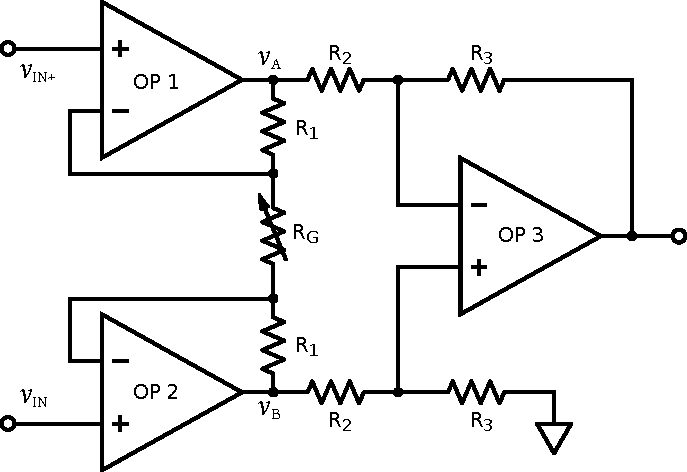
\includegraphics[width=0.350\textwidth]{../E05/latex/c_INA.pdf}
  \end{center}
  \caption{Circuito dell'amplificatore per strumentazione.}
  \label{cir5:instr_amplif}
\end{wrapfigure}


Verifichiamo invece che la resistenza posta in mezzo varia effettivamente il guadagno del circuito. Dividiamo il circuito in due parti, calcolandoci prima la tensione fra il punto A e B\footnote{Si noti che un circuito che abbia come $V_{out}$ la differenza fra questi due punti sarebbe flottante sull'uscita. Infatti, una eventuale resistenza di carico messa fra il punto A e B non avrebbe un riferimento di comune.}, per poi la tensione di uscita dell'intero circuito. Per la prima parte, considerando i due operazionali ideali, otteniamo che le tensione agli ingressi invertenti sono $V_{OP_1}^- = V_1$ e $V_{OP_2}^- = V_2$. Dunque ai capi di $R_g$ è presente una differenza di potenziale $V_2-V_1 = \Delta V_{in}$; per l'idealità degli OPAMP, abbiamo inoltre che la corrente che passa per le resistenze $R_1$ ed $R_g$ sono uguali. Otteniamo dunque, sommando le cadute di potenziale
$$\Delta V_{AB} = \frac{\Delta V_{in}}{R_g} R_g + \frac{\Delta V_{in}}{R_g} R_1 + \frac{\Delta V_{in}}{R_g} R_2$$
cioè
\begin{equation}
\Delta V_{AB} = \Delta V_{in} \left(1+\frac{2R_1}{R_g}\right)
\label{eq5:TEMP_calcoli}
\end{equation}

Valutiamo ora la seconda parte del circuito data da $OP_3$. Per quanto riguarda la tensione all'ingresso non invertente, questa è data da un semplice partitore (non scorre corrente nell'ingresso dell'opamp)
$$V^+=V_B \frac{R_3}{R_3+R_2}$$
All'ingresso non invertente vale invece la legge di Kirkhhoff per i nodi
$$\frac{V_A-V^-}{R_2}+\frac{V_{out}-V^-}{R_3}=0$$
da cui
$$V^-=V_A \frac{R_3}{R_2+R_3} + V_{out} \frac{R_2}{R_2+R_3}$$

Uguagliando $V^-$ e $V^+$ (OPAMP ideale), tenendo conto della (\ref{eq5:TEMP_calcoli}), otteniamo dunque
$$V_{out}=-\Delta V_{in} \left(1+\frac{2R_1}{R_g}\right)\frac{R_3}{R_2}$$
Modificando la resistenza $R_g$ possiamo dunque controllare il guadagno del circuito.

\subsubsection{Integrato AD622}

\begin{wrapfigure}[14]{l}{0.5\textwidth}
  \begin{center}
    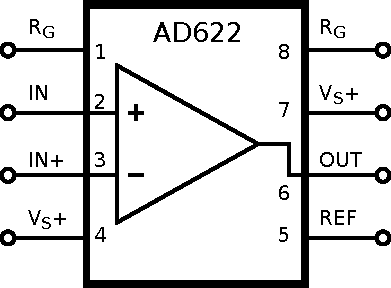
\includegraphics[width=0.260\textwidth]{../E05/latex/AD622.pdf}
  \end{center}
  \caption{Piedinatura dell'integrato AD622.}
  \label{cir5:ad622_piedinatura}
\end{wrapfigure}

In realtà, nell'esperienza abbiamo utilizzato un circuito integrato (più precisamente l'AD622, la cui piedinatura è esposta in Figura \ref{cir5:ad622_piedinatura}) che ha come qualità il fatto di avere un'alta precisione sul valore delle resistenze (abbiamo visto nel precedente circuito che uno squilibrio anche minimo fra i valori di resistenze che dovrebbero essere uguali può portare ad un guadagno diverso da quello teorico). Il suo guadagno è dato dall'equazione, fornita dal costruttore
$$G=1+\frac{50.5 \si{\kilo\ohm}}{R_g}$$

Una possibile applicazione di questo integrato è di utilizzarlo per individuare variazioni di tensione all'interno di un ponte di resistenze. Allo scopo, utilizziamo il circuito in Figura \ref{cir5:ad622_ponte}, con l'accortezza di portare una resistenza del ponte lontana dalle altre, così da poter modificarne la temperatura senza influenzare anche le altre.

Infatti, sappiamo che le resistenze hanno una dipendenza dalla temperatura data dal coefficiente di temperatura, che è di circa $200$ ppm/\si{\celsius}. Nel nostro caso, utilizzando come resistenza lontana dalle una da $100$ \si{\ohm}, la sua variazione per grado di temperatura sarà di $\Delta R / \Delta T= 100 \si{\ohm} (-200 \times 10^{-6}) = -20$ \si{\milli\ohm/\celsius}. Inoltre, per il ponte vale che non vi è differenza di tensione fra gli ingressi dell'integrato se il prodotto delle resistenze $R_1 R_4=R_2 R_3$: dunque, variando la resistenza $R_3$ inizieremo a registrare una tensione di uscita.

Sperimentalmente, si osserva però che una differenza di potenziale è già presente a temperatura ambiente (cioè senza variare la temperatura della resistenza $R_3$): questo fatto è imputabile al mancato bilanciamento del ponte. Infatti, è impossibile trovare due resistenze che abbiano un valore esattamente identico: dunque vi è un errore sistematico di cui dobbiamo tenere conto prima di effettuare le misure, fissando un valore zero di tensione, che si osserva essere $0.54$\si{\volt}.

Inoltre, la relazione che lega la variazione di tensione alla resistenza può essere calcolata considerando il ponte come l'insieme di due partitori (non scorre alcuna corrente verso l'amplificatore), cioè vale che
$$\Delta V = V^+ - V^- = V_d \left(\frac{R_4}{R_2+R_4}-\frac{R_2}{R_1+R_3}\right)$$

\begin{wrapfigure}[20]{r}{0.5\textwidth}
  \begin{center}
    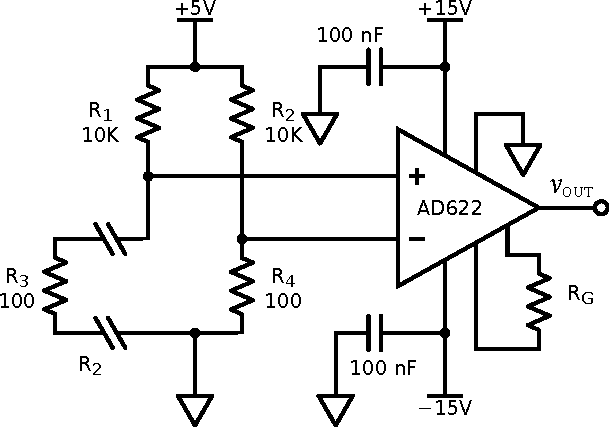
\includegraphics[width=0.40\textwidth]{../E05/latex/c_func_INA.pdf}
  \end{center}
  \caption{Circuito del ponte con l'amplificatore per strumentazione AD622. Le capacità sono state poste fra l'alimentazione e terra come per il $\mu$741.}
  \label{cir5:ad622_ponte}
\end{wrapfigure}

Considerando che l'uscita è amplificata dall'AD622 di un fattore di guadagno $A \approx 1000$ e $R_4/R_1<<1$, svolgendo i calcoli per $R_3=R_4+\Delta R$, otteniamo la seguente equazione
\begin{equation}
\Delta V_{out} = - A \frac{\Delta R}{R_1+R_4} V_{b}
\label{eq5:delta_R}
\end{equation}
dove $V_{b}$ è la tensione di alimentazione del ponte (come in Figura \ref{cir5:ad622_ponte}). Tenendo conto della relazione fra $\Delta R$ e la variazione di temperatura $\Delta T$, abbiamo che
\begin{equation}
\Delta T = \frac{\Delta R}{- 20 \si{\milli\ohm/\celsius}} = \frac{1}{20 \si{\milli\ohm/\celsius}} \frac{R_1+R_4}{V_b A} \Delta V
\label{eq5:delta_T}
\end{equation}

Presentiamo ora la tabella dei valori sperimentali con la modalità di variazione della temperatura. I valori di $\Delta V$ sono osservati, $\Delta R$ e $\Delta T$ sono calcolati rispettivamente con (\ref{eq5:delta_R}) e (\ref{eq5:delta_T}).

$$$$

\begin{center}
{\renewcommand{\arraystretch}{1.2}%
	\begin{tabular}{c|c|c|c}
    %\hline
	Modalità & $\Delta V$ [\si{\volt}] & $\Delta R$ [\si{\ohm}] & $\Delta T$ [\si{\celsius}]\\
    \hline
	Soffio & $0.08\pm0.01 $ & $0.16\pm0.02$ & $8 \pm 1$\\
    \hline
	Refrigerante & $-0.44\pm0.02 $ & $-0.88\pm0.07$ & $-44 \pm 3$\\
    %\hline
	\end{tabular}
}
\end{center}

\subsection{Misure di temperatura}

\begin{wrapfigure}[13]{r}{0.45\textwidth}
\centering
\caption{Circuito di controllo della temperatura a distanza: PT100 è il termoresistore al platino, l'ohmetro misura la resistenza in funzione della temperatura e le due resistenze da \SI{10}{\ohm} simulano i cavi lunghi.}
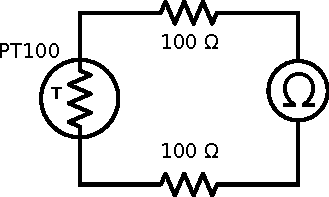
\includegraphics[width=.25\textwidth]{../E05/latex/c_PT100_2wire.pdf}
\label{cir5:2wire}
\end{wrapfigure}

Nell'ultima parte dell'esperienza abbiamo eseguito misure di temperatura utilizzando una termoresistenza al platino PT100.
Essa non è altro che una resistenza di cui sono noti con sufficiente precisione alcuni parametri: il valore ad una data temperatura e il coefficiente di temperatura $\alpha$.

Sapendo che il valore di resistenza è dipendente dalla resistività elettrica del materiale $\rho$ che a sua volta dipende dalla temperatura (nel caso di metalli), secondo le seguenti relazioni:
	$$	R = \frac{\rho L}{S}
			\qquad \qquad
		\rho = \rho_0 \left[ 1 + \alpha \left( T - T_0 \right) \right]$$
dove L è la lunghezza del materiale e S la sezione, mentre $\rho$ dipende dalla resistività $\rho_0$ alla temperatura di riferimento $T_0$ e dal coefficiente di temperatura $\alpha$.
Combinando le due equazioni precedenti si ottiene la dipendenza del valore di resistenza dalla temperatura:
\begin{equation}
R = R_0 \left[ 1 + \alpha \left( T - T_0 \right) \right]
\end{equation}



Invertendo la formula si ottiene:
\begin{equation}
T = T_0 + \frac{1}{\alpha}\left( \frac{R}{R_0}-1 \right)
\end{equation}
Nel nostro caso il costruttore ci ha fornito i dati relativi alla temperatura di riferimento $T_0 =$ \SI{0}{\degreeCelsius}:
$$R_0 = \SI{100}{\ohm} \quad \quad \alpha = \SI{0.003850}{\per\degreeCelsius}$$

Conoscendo il comportamento della termoresistenza abbiamo simulato il caso in cui si volesse controllare la temperatura di un laboratorio a distanza.
I circuito che simulava questa situazione è riportato in Figura \ref{cir5:2wire}

Abbiamo notato subito che le misure ricavate con questo circuito soffrivano dell'errore sistematico dato dalle resistenze in serie da \SI{10}{\ohm}.
Infatti il valore di resistenza letto dall'ohmetro era di \SI{130}{\ohm}, che dava in risultato una temperatura ambiente di $\approx$ \SI{78}{\degreeCelsius}, evidentemente errata.


\begin{wrapfigure}[14]{l}{0.45\textwidth}
\centering
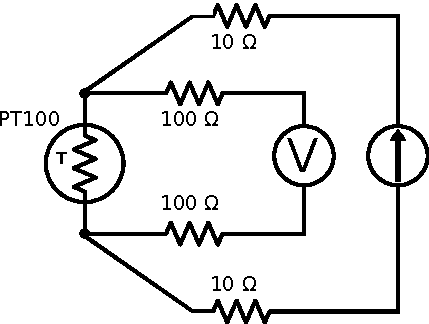
\includegraphics[width=.25\textwidth]{../E05/latex/c_PT100_4wire.pdf}
\caption{Configurazione di misura a quattro fili: nella maglia esterna scorre la corrente data dal generatore mentre nella maglia interna non scorre corrente. Il voltmetro ha un'impedenza idealmente infinita.}
\label{cir5:4wire}
\end{wrapfigure}

Per evitare questo tipo di problemi abbiamo effettuato una misura a quattro fili.
In questa modalità il multimetro funzionava come generatore di corrente costante tramite due boccole e da voltmetro con le altre due boccole utilizzate.
Lo schema riportato in Figura \ref{cir5:4wire} mostra come la misura questa volta sia effettuata acquisendo la differenza di potenziale ai capi della termoresistenza data dalla corrente del generatore.
In questa configurazione non vi è l'errore sistematico della misura a due fili, in quanto grazie all'alta impedenza del voltmetro, nella maglia interna non scorre corrente e pertanto ai capi delle resistenze su tale maglia non vi è alcuna caduta di potenziale.

Nella tabella seguente sono riportati i valori per $T_0 =$ 0, per due temperature vicine alla temperatura ambiente, per una temperatura ottenuta raffreddando con una bomboletta di refrigerante e riscaldando il termoresistore a temperatura corporea.

\begin{center}
{\renewcommand{\arraystretch}{1.4}%
\begin{tabular}{c|c c c c c}
$R$ [\si{\ohm}] 		& $R_0 =$ 100 	& 110.24 & 111.32 & 83.37 & 114.71\\ 
\hline 
$T$ [\si{\degreeCelsius}] 	& $T_0 =$ 0 	& 26.6 & 29.4 & -43.2 & 38.2 \\ 
\end{tabular}}
\end{center}

\subsection*{Conclusioni}
In questa esperienza abbiamo studiato alcuni circuiti utili a trasformare un segnale senza modificare l'informazione in esso contenuta: in particolare abbiamo esaminato circuiti raddrizzatori che non diminuiscono l'ampiezza del segnale come accade con i circuiti passivi quali i semplici diodi o il ponte raddrizzatore (ponte di Graetz).

Successivamente abbiamo studiato il cosiddetto amplificatore da strumentazione, in un circuito didattico costruito con un $\mu$A741 le cui limitazioni sono date dal guadagno fisso e dalla bassa impedenza in entrata e integrato in un dual inline package (AD622).
Ne abbiamo testato il funzionamento misurando lo sbilanciamento di un ponte di Wheatstone.

Infine abbiamo studiato le problematiche di una misura di temperatura a distanza data dalla lunghezza dei cavi. Abbiamo risolto utilizzando un sistema di misura a quattro fili.
